Die Ortsänderung ist die Fläche unter dem $v(t)$-Graphen, über der $t$-Achse positiv, unter der Achse negativ.
\begin{center}
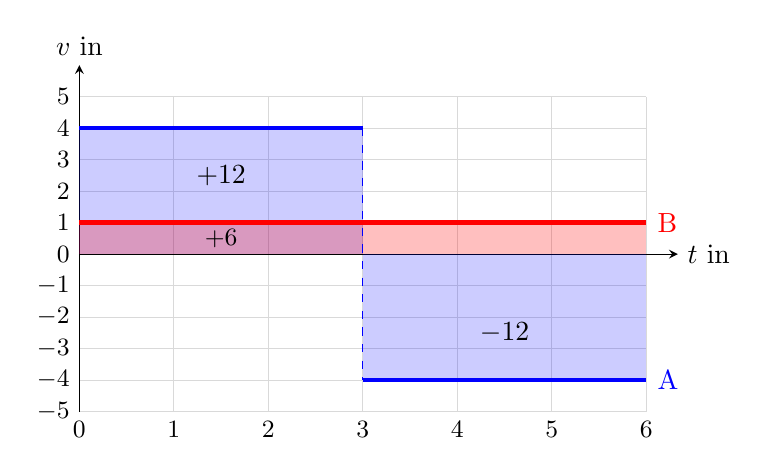
\begin{tikzpicture}[>=stealth, x=1.2cm, y=0.4cm]
 \draw[gray!30] (0,-5) grid[xstep=1, ystep=1] (6,5);
 \draw[->] (0,0) -- (6.333,0) node[right] {$t$ in \si{\second}};
 \draw[->] (0,-5) -- (0,6) node[above] {$v$ in \si{\meter\per\second}};
 \foreach \tk in {0,1,2,3,4,5,6} \node[below] at (\tk,-5) {\small $\tk$};
 \foreach \yk in {-5,-4,-3,-2,-1,0,1,2,3,4,5} \node[left] at (0,\yk) {\small $\yk$};

 \fill[blue, opacity=0.2] (0,0) rectangle (3,4);
 \fill[blue, opacity=0.2] (3,0) rectangle (6,-4);
 \fill[red, opacity=0.25] (0,0) rectangle (6,1);
 \draw[ultra thick, blue] (0,4) -- (3,4);
 \draw[blue, dashed] (3,4) -- (3,-4);
 \draw[ultra thick, blue] (3,-4) -- (6,-4) node[right] {A};
 \draw[ultra thick, red] (0,1) -- (6,1) node[right] {B};
 \node at (1.5,2.5) {$+12$};
 \node at (4.5,-2.5) {$-12$};
 \node at (1.5,0.5) {\small $+6$};
\end{tikzpicture}
\end{center}
\begin{abcliste}
\abc
\begin{align}
 s_\mathrm{A} &= \sAF = \vA\cdot\tH-\vA\cdot\left(\tE-\tH\right) = \sA \approx \result{\SI{0}{\meter}} \\
 s_\mathrm{B} &= \sBF = \vB\cdot\tE = \sB \approx \result{\sBP{0}{1}}
\end{align}
A ist wieder am Start.

\abc $\result{\text{B}}$ ist weiter vom Startort entfernt.

\abc Noah verwechselt die zurückgelegte Strecke mit der Ortsänderung. A legt zwar
\begin{align}
 d_\mathrm{A} &= \dAF = \dA \approx \dAP{0}{2}
\end{align}
zurück, die Hälfte davon aber rückwärts. Für die Entfernung vom Start zählt die Fläche unter der Achse negativ: \SI{12}{\meter} hin und \SI{12}{\meter} zurück ergibt $\Delta s = 0$. B fährt nur \sBP{0}{1}, aber immer in dieselbe Richtung.
\end{abcliste}
